\documentclass[14pt, a4paper]{article}

\usepackage[T2A]{fontenc}
\usepackage[utf8]{inputenc}
\usepackage[english, russian]{babel}

\usepackage{amsmath}
\usepackage{float}
\usepackage{graphicx}
\graphicspath{{./images/}}

\begin{document}
    \thispagestyle{empty}

    \begin{center}
        Министерство науки и высшего образования Российской Федерации

        Федеральное государственно автономное образовательное учреждение высшего образования

        <<Омский государственный технический университет>>

        \vspace{1cm}
        Факультет информационных технологий и компьютерных систем

        Кафедра <<Прикладная математика и фундаметральная информатика>>

        \vspace{3cm}
        \textbf{Лабораторная работа №6}

        по дисциплине <<Компьютерные сети>>
    \end{center}
    
    \vspace{3cm}
    \begin{flushright}    
        \begin{tabular}{ r r }
            Студента & Курпенова Куата Ибраимовича \\
            \cline{2-2}
            & \tiny{фамилия, имя, отчество полностью} \\

            Курс & 2, группа ФИТ-212 \\
            \cline{2-2}
            Направление & 02.03.02 Прикладная математика \\
            \cline{2-2}
            & и фундаментальная информатика \\
            \cline{2-2}
            & \tiny{код, наименование} \\
            
            Руководитель & ст. преподаватель \\
            \cline{2-2}
            & \tiny{должность, ученая степень, звание} \\
            & Литвинов Г. А. \\
            \cline{2-2}
            & \tiny{фамилия, инициалы} \\
            
            Выполнил & \\
            \cline{2-2}
            & \tiny{дата, подпись студента(ки)} \\

            Проверил & \\
            \cline{2-2}
            & \tiny{дата, подпись преподавателя} \\
        \end{tabular}
    \end{flushright}
    
    \vspace*{\fill}
    \begin{center}
        Омск 2022
    \end{center}

    \newpage

    \section*{Решение}

    \begin{figure}[H]
        \centering
        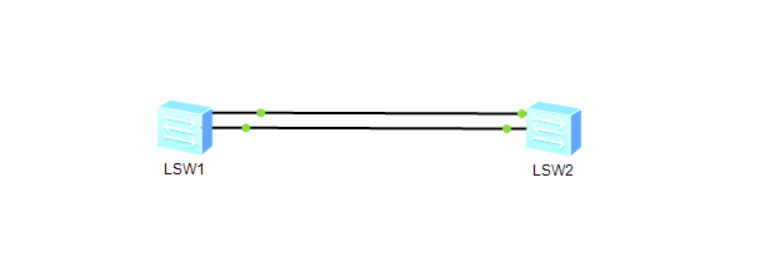
\includegraphics[width=\textwidth]{images/scheme.png}
        \caption{Схема свитчей}
    \end{figure}

    \begin{figure}[H]
        \centering
        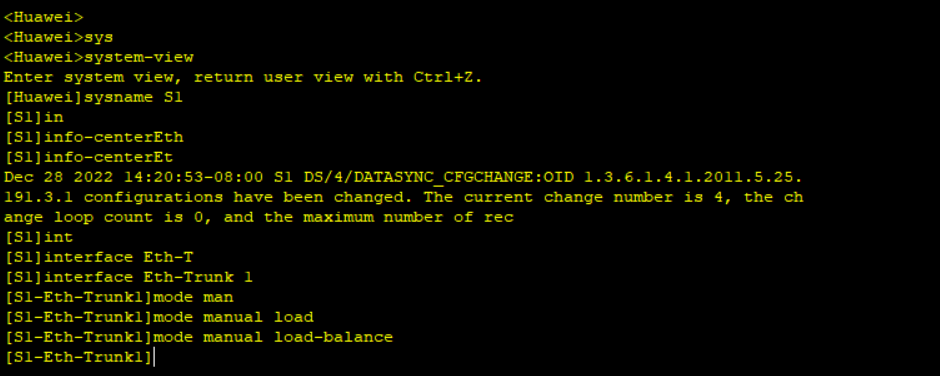
\includegraphics[width=\textwidth]{images/trunk_s1.png}
        \caption{Установка Eth-Trunk на switch 1}
    \end{figure}

    \begin{figure}[H]
        \centering
        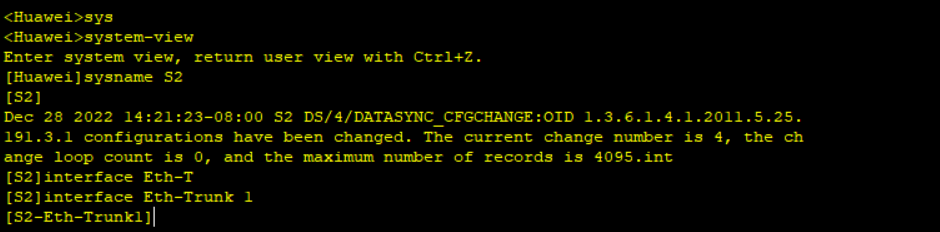
\includegraphics[width=\textwidth]{images/trunk_s2.png}
        \caption{Установка Eth-Trunk на switch 1}
    \end{figure}

    \begin{figure}[H]
        \centering
        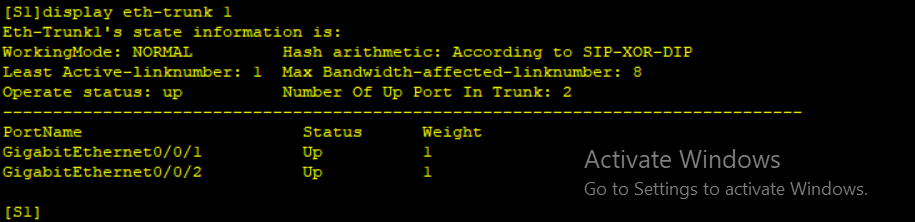
\includegraphics[width=\textwidth]{images/display_trunk.png}
        \caption{Схема Eth-Trunk}
    \end{figure}

    \begin{figure}[H]
        \centering
        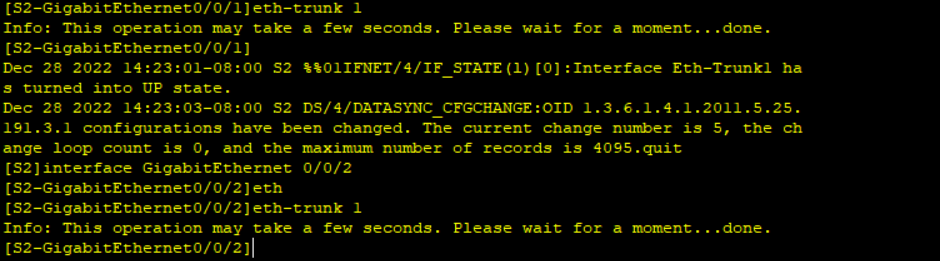
\includegraphics[width=\textwidth]{images/trunk_connect_s1.png}
        \caption{Trunk connect switch 1}
    \end{figure}

    \begin{figure}[H]
        \centering
        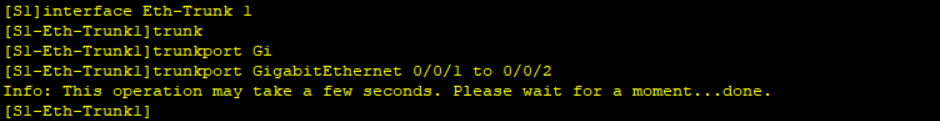
\includegraphics[width=\textwidth]{images/trunkport.png}
        \caption{Схема Trunkport}
    \end{figure}

    \begin{figure}[H]
        \centering
        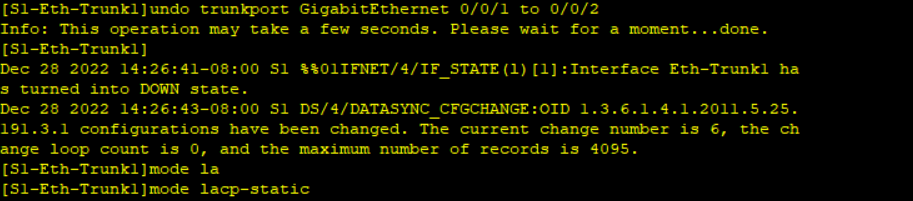
\includegraphics[width=\textwidth]{images/trunkport_disable.png}
        \caption{Trunkport disable}
    \end{figure}
\end{document}
